%
%   Main Text for  Forschergruppenproposal
%    The Formation of Planets
%         May 2006
%
\section{Participating institutes and 
principle investigators
%\footnote{Only PIs and Co-PIs listed. Co-investigators and 
%collaborators are listed in individual projects.}
}\label{app-institutes}
\vspace{0.1em}
\renewcommand{\hdrtitle}{Participating institutes and PIs}
\begin{itemize}
\item {\bf University of T\"ubingen:}
\begin{compactitemize}
  \item Institute for Astronomy \& Astrophysics \\
%%    Dept.~of Computational Physics \\
         {\em (Prof.~Dr.~W.~Kley, Dr.~R.~Speith)}
\end{compactitemize}
\item {\bf University of Heidelberg:}
  \begin{compactitemize}
  \item Institute for Theoretical Astrophysics\\
         {\em (Prof.~Dr.~W.~M.~Tscharnuter, Prof.~Dr.~H.-P.~Gail)}
  \item Mineralogical Institute \\
         {\em (Dr.~M.~Trieloff, Prof.~Dr.~D.~Lattard, Prof.~Dr.~R.~Altherr)}
  \item Kirchhoff Institute of Physics, group ``Surface Science and
         Infrared Spectroscopy of Nanostructures'' \\ {\em
         (Prof.~Dr.~A.~Pucci)}
  \end{compactitemize} 
\item {\bf Max-Planck-Institute for Astronomy, Heidelberg:}
\begin{compactitemize}
  \item Planet and Star Formation Group\\
         {\em (Dr.~H.~Klahr, Dr.~C.~P.~Dullemond, Prof.~Dr.~Th.~Henning)}
  \item Emmy Noether Group ``Evolution of circumstellar dust disks to
         planetary systems''\\
         {\em (Dr.~S.~Wolf)}
\end{compactitemize}
\item {\bf Technical University at Braunschweig:}
\begin{compactitemize}
  \item Institute for Geophysics and Extraterrestrial Physics \\
         {\em (Prof.~Dr.~J.~Blum)}
\end{compactitemize}
\item {\bf University of M\"unster:}
\begin{compactitemize}
  \item Emmy Noether Group ``Dust, Gas, Radiation and Planet Formation''\\
         {\em (Dr.~G.~Wurm)}
  \item Institute of Planetology\\
         {\em (T. Stephan)}
\end{compactitemize}
\end{itemize}
%
%\mbox{}\vspace{0.2em}\\
%
\noindent {\bf Speaker:}\\
%%\noindent Prof.~Dr.~W.~M.~Tscharnuter \hfill Tel.: 06221-544815\\
%%Zentrum f\"ur Astronomie, Uni-HD \hfill e-mail wmt@ita.uni-heidelberg.de\\
%Institut f\"ur Theoretische Astrophysik\\
%Universit\"at Heidelberg, \\
%%Albert-\"Uberle-Str. 2, D-69120 Heidelberg\\
%%  New since April 2006 
\noindent Prof.~Dr.~W.~Kley \hfill Tel.: 07071-29-74007\\
University of T\"ubingen \hfill 
E-mail: wilhelm.kley@uni-tuebingen.de\\
Institute for Astronomy \& Astrophysics \\
Auf der Morgenstelle 10, D-72076 T\"ubingen\\[1em]

\noindent {\bf Co-speakers:}\\
\noindent Dr.~C.~P.~Dullemond \hfill Tel.: 06221-528-395\\
Max-Planck-Institute for Astronomy\hfill 
E-mail: dullemon@mpia.de\\
K\"onigstuhl 17, D-69117 Heidelberg\\[0.1em]

\noindent Dr.~M.~Trieloff \hfill Tel.: 06221-546022\\
Mineralogical Institute \hfill E-mail: trieloff@min.uni-heidelberg.de\\
University of Heidelberg \\
Im Neuenheimer Feld 236, D-69120 Heidelberg


\pagebreak[4]


\section{Summary}
\renewcommand{\hdrtitle}{Summary}
The formation of planets is one of the key questions in astrophysics. The
first step in this process is the coagulation of dust: the growth from
sub-micron dust particles to ever larger aggregates ultimately leading to
the formation of multi-kilometer sized `planetesimals'. Once these
planetesimals are formed, gravitational interaction starts to dominate over
all other forces, and eventually leads to the formation of rocky planets.
In our proposed Forschergruppe we focus on the {\it first stage} in the planet
formation scenario, i.e. on the growth process from dust to planetesimals.
 
This stage suffers from a large number of
unsolved mysteries, many of which are critical to our understanding of the
planetesimal formation process as a whole.  
Among them are: The seemingly insurmountable
`meter-size barrier' for the collisional growth of particles, the poorly
understood causes of the complex mineralogical structure of meteorites, and
the apparent lack of correlation between certain observational signatures of
grain evolution and the age of the parent star. In spite of the clear
connection between these issues, they have mostly been studied by somewhat
separate scientific communities. In particular the
meteoritics/cosmochemistry/astromineralogy community, the collision
experimentalists, the theoretical astrophysicists and the observational
astronomers have had relatively little cross-field collaboration in the past. 
The most promising option to solve many questions surrounding the growth from dust to
planetesimals is to unite these various communities in a joint research
effort. This is the purpose of the proposed Forschergruppe.


\section{Introduction and motivation}
\renewcommand{\hdrtitle}{Introduction} Understanding the formation of
planets is of such importance because it relates to the foundation of our
own existence, and whether planets such as our Earth are rare or common in
the Milky Way. Although it is one of the oldest questions in astronomy and
of mankind, it has recently attained strong renewed interest stimulated by
the discovery of over 180 extrasolar planets around solar-type stars in the
last decade. Improved observational sensitivity has allowed to detect objects
as small as Neptune (14 Earth masses), and through transit observations
physical properties of extrasolar planets such as radius and mean density
have been inferred.  Moreover, with the newest infrared telescope
facilities, the birthplaces of planets - the dusty protoplanetary
circumstellar disks left over from the star formation phase - can now be
studied to an unprecedented level of detail, allowing astronomers and
astrophysicists to put theories of planet formation to the test. The near
future also promises interesting new views on this issue: it is expected
that within 10 years {\em earth-like} extrasolar planets will have been
discovered with space missions, which will put new constraints on the
scenarios of formation of planets such as our own.

Planet formation is believed to begin with the coagulation of dust in
protoplanetary disks, forming ever larger aggregates of solid material through
a sequence of collisions and agglomerations. This growth process 
continues until eventually these bodies become gravitationally bound
objects of a few kilometers in size. This initial phase of planet formation
constitutes a growth over 10 orders of magnitude in size and over 30 orders
of magnitude in mass. It is a process of high complexity involving many
aspects of physics, chemistry, astronomy and mineralogy. These aspects
include the physics of colliding aggregates, the internal structure of
aggregates, the solid-state chemistry of grains at high temperatures, the
interaction between grains and the surrounding gas and hydrodynamic flows,
and the large-scale evolution of dust populations. The study of these
processes also requires knowledge on the structure and evolution of the
disks in which these processes take place, including the transport of
radiation through these disks. Moreover, the evolving dust population has a
back reaction on the structure of these disks. A comprehensive study of the
growth process from sub-micron dust particles to multi-kilometer planetesimals is
therefore a problem of such complexity that its study requires a large
collaborative effort between scientists with expertise in all these various
mutually-interacting aspects of this problem.
 
%
\subsection{Why study {\em this} stage of planet formation?}
\label{subsec:whynow}
%
Although the {\em entire} process of planet formation is highly relevant,
the first stage --the growth from dust to planetesimals-- is of particular
interest. There are three main reasons for this: {\it 1)} 
This is probably the observationally best constrained part of the planet
formation theory, with a wealth of infrared and sub-millimeter data from 
hundreds of protoplanetary disks, and the additional detailed meteoritic knowledge of
our own Solar System. {\it 2)} This is the stage of planet formation that
links the origin of asteroids and comets to the origin of planets, and which
gives a comprehensive view on the formation of rocky planets. {\it 3)} 
It involves many unsolved critical questions about planet formation in areas of
expertise of our team.

Many of these questions are so fundamental that to this date there 
exists no standard scenario of how this process operates. For instance, it is
not known how particles survive the `meter-size barrier', a size-regime in
which relative velocities are so large that a collision with an equal-sized
body would completely destroy both objects. Moreover, according to simple
physical arguments, bodies of this size should drift very rapidly
towards the star, vaporize, and therefore get lost for the planetesimal
formation process. Even putting these issues aside, it is still not known
{\em how} bodies grow to planetesimal sizes. Is it a hierarchical growth
process, or do the biggest bodies grow by sweeping up large quantities of
dust and small bodies? Under which conditions are
these impacts constructive and when are they erosive?  Does the growth take
place everywhere in the whole disk, or does it require an essential
boost through some triggering mechanisms such as hydrodynamic clustering of
particles in vortices and/or turbulent eddies?

These are only a few of the fundamental unsolved questions concerning the
theory of particle growth and planetesimal formation.  When considering the
{\em composition} and size-distribution of these particles, as measured by
infrared observations of protoplanetary disks and (in even more detail) by
meteoritic studies of our own Solar System, one is confronted by an equally
puzzling --and similarly vast-- set of additional mysteries.  For instance,
it is a hotly debated issue why the elementary composition of chondrules -
millimeter sized crystalline globules of which chondritic meteorites are
largely built up - is complementary to that of the fine grained matrix
particles between chondrules, and what is the reason for compositional
variety of chondrite parent bodies.  Furthermore, it is unclear why
Calcium-Aluminum-rich Inclusions (CAIs) are a few million years older than
most chondrules from the same meteorites, and why differentiated meteorites
are nearly as old as CAIs and hence, older than chondrites and
chondrules. The composition of comets is also enigmatic - though there are
likely cometary particles (fluffy, anhydrous) in collected interplanetary
dust samples, it is unclear, why these contain mostly isotopically normal,
solar dust. Here, soon progress is expected by the Stardust mission.  Also
from observations of protoplanetary disks there are many puzzles, for
instance: why do signatures of grain growth and thermal processing
(crystallinity) not appear to be correlated with the stellar age? Is there
another parameter in addition to stellar age?
%

\subsection{Why study it {\em now}?}
%
Three recent ground-breaking new developments have improved our
understanding of this topic, and are major motivations for the
Forschergruppe:

\noindent {\it 1)} There is enormous progress in infrared astronomy, in
particular in the spectroscopic study of dust particles in protoplanetary
disks around Herbig Ae/Be stars, T Tauri stars, and Brown Dwarfs. For many
years the Hubble Space Telescope has provided us with outstanding images and
spectra, and since 2004 the {\em Spitzer Space Telescope} yields enormous
quantities of data on the dust grain sizes and composition in infant `Solar
Systems'. Its unprecedented sensitivity allows, for the first time, a
detailed look at the infrared spectra of dim sources such as T Tauri stars
(among which are infant sun-like stars) and even Brown Dwarfs. Moreover, the
sample of sources with good spectra has increased dramatically with this
telescope, so that detailed statistical studies can be done. In addition to
this, since 2003 the Very Large Telescope (ESO, Chile) can spatially resolve
the very inner regions of protoplanetary disks where Earth-like planets may
form, and analyze grain sizes and composition as a function of distance from
the star down to spatial scales of about 1 AU.  And finally, in recent years
there have been major breakthroughs in millimeter interferometry
measurements of protoplanetary disks. With these measurements it has been
established that large quantities of few-millimeter sized pebbles reside in
the midplane of these disks out to many tens of astronomical units, posing
problems to theories of grain motion. Moreover, sometimes this mm/cm size
grain population can been shown to have a very narrow size distribution,
which is a puzzle for theoretical models.
%  The Max Planck Institute for Astronomy
% (MPIA) in Heidelberg has a large team of scientists working on the analysis
% of these data in order to gain insight on the growth and thermal/chemical
% processing of dust grains in protoplanetary disks.

\noindent {\it 2)} 
In recent years there has been major progress in
laboratory experiments of collisions of dust aggregates. With these
experiments our knowledge of the sticking coefficients, the structure of
aggregates, and the typical (debris-) products of collisions are now much
better known than a decade ago. These microphysical data are the basic
physical ingredients for models dealing with the evolution of the grain size
distribution in protoplanetary disks. New and improved coagulation models
can therefore be developed based on these data, and the above mentioned
questions can be addressed with more reliable and realistic tools.
% The Laboratories in Braunschweig and M\"unster have played a major
% role in these developments.

\noindent {\it 3)} 
The last decade brought enormous progress in micro- and
nano-analytics of extraterrestrial matter and advances in establishing the
chronology of early Solar System processes, particularly regarding the
growth of asteroid-sized planetesimals.
%
The STARDUST mission - the first sample return mission since the Apollo
program - just brought back cometary dust from comet Wild-2. The analysis of
this most primitive matter has started and is expected to significantly
increase our knowledge about the formation of the first small bodies in our
solar system.
%
It is tantalizing to compare what we
know from our own Solar System with results from infrared observations of
protoplanetary disks, and to try to match theories of grain growth to these
observations. In this way, both our own Solar System, as well as
proto-solar-systems in our neighborhood may be able to provide new clues to
the growth of planetesimals.



\subsection{Why do we need a Forschergruppe?}
%
The problem of the formation of planetesimals involves many different
processes which are often studied by very different communities. While the
formation of our own Solar System is studied by meteoritic scientists, the
observations of protoplanetary disks are performed by observational
astronomers. And while the collisions of aggregates are studied in the lab
by laboratory astrophysicists, the mineralogical composition of these grains
is studied by cosmochemists.
%
% KEES: Cosmochemists?
%

Yet, it is evident that all these aspects are strongly intertwined. Each of
these aspects has so far been studied mostly in isolation, but this was
only possible because drastic simplifying assumptions have been made for the
other aspects. For instance, the materials used for aggregates in laboratory
collision experiments were mostly quartz spherules, while we know that a
whole variety of different minerals must have been present in the early solar nebula.
Models of grain growth often use a relatively primitive coagulation kernel,
while lab experiments have demonstrated its immense
complexity. Interpretation of infrared observations often employs models
with simple power-law grain size distributions, while theory clearly shows
that grain size distributions differ substantially from a power-law.

{\em Only by studying all aspects in a unified way there is hope that real
progress can be made, and the main unexplained problems be solved.} Since
isolated research efforts cannot cover all these aspects, it is clear that
such a study requires a close collaborative project involving experts from
all these aspects of planetesimal formation. The initiation of such a joint scientific
effort combining different research fields is one of our main goals to achieve
with this Forschergruppe. 

%\pagebreak[4]

\section{Scientific background and own contributions}
\renewcommand{\hdrtitle}{Scientific background}
%
In the following subsections we will summarize the state of the various
areas of research mentioned in the introduction and own contributions in these.

\subsection{Disk structure and evolution:}
%
Though disk structure and evolution is not the topic of this Forschergruppe,
the physics of planetesimal formation takes place within such disks. For
this reason our expertise on this topic plays an important role in this
Forschergruppe, and we will concisely list our contributions to this field
below.  But since this field is quite extensive, and not within the main
focus of this Forschergruppe (it only plays a passive supportive role), we
do not review the current status of this field here. For recent reviews see
e.g.~D'Alessio et al.~(\cit{2005}) and Dullemond et al.~(\cit{2006}).

\paragraph{Our contributions:}
%
The detailed 2-D global structure of irradiated protoplanetary disks has
been studied by Dullemond et al.~(\cit{2002, 2003, 2004b}).  Hydrodynamic
and radiative transfer models for disks are also available within the group
of Gail \& Tscharnuter (Gail \cit{2001, 2003, 2004}; Wehrstedt \&
Gail \cit{2002, 2003}), as well as in the groups of Klahr and Henning (Bell
et al.~\cit{1997}; Klahr et al.~\cit{1999, 2003, 2005}; W\"unsch et
al.~\cit{2005}) and of Kley (Kley et al.~\cit{2001}; G\"unther et
al.~\cit{2002, 2004}; Sch\"afer et al.~\cit{2004}). Models of the ionization
of disks, with particular relevance to the magneto-rotational instability,
have been constructed by Semenov \& Henning (\cit{2004}).  Models of the
formation and viscous evolution, based on time-dependent $\alpha$-disk
equations, were published by Dullemond et al.~(\cit{2006a}, \cit{2006b}).


\subsection{Thermal processing and radial mixing}
%
Cometary nuclei contain ices, refractory organics and silicate dust grains
(Jessberger et al. 1988; Jessberger 1999). Recent observations made clear
that, in addition to amorphous dust, such comets also contain a considerable
fraction of crystalline Mg-rich silicate dust species (e.g.\ Wooden et
al.~\cit{1999, 2000, 2004}). Such dust species are can only be created at
temperatures exceeding 800 K. The coexistence of this high temperature
material with amorphous dust in the same objects points to large scale
radial mixing/transport processes in protoplanetary disks
(e.g.~Bockel\'ee-Morvan et al.~\cit{2002}; Nuth \& Johnson \cit{2006}),
although shocks have also been discussed (e.g.\ Harker \& Desch \cit{2002};
Miura \& Nakamoto \cit{2005}). Such processes are important for the disk
structure and its material, as well as for the composition of the planets
and planetesimals formed in the disk (e.g.~Morfill, Tscharnuter \& V\"olk
\cit{1985}).

Crystalline silicate dust is also detected in protoplanetary disks
(e.g.~Meeus et al.~\cit{2001}; Bouwman et al.~\cit{2001}; Apai et
al.~\cit{2005}). For three such sources, the 'Mid-Infrared Interferometric
Instrument' (MIDI) has recently obtained mid-infrared spectra of the disk at
different stello-centric radii (\coll{van Boekel et al.~\cit{2004}}).  These
observations clearly show a radial decrease of the degree of crystallization
of the dust in the disk, which points to radial mixing theories. But it
remains a puzzle why some sources have significantly more crystalline dust
than others. 
% {\bf [****** STATEMENT REMOVED ******]}
%, and how it can be that some sources appear to have virtually no
%crystalline silicates just outside of the thermal annealing radius (indicating
%zero mixing).

%\remark{INSERT EVAPORATION CONDENSATION}
Besides the crystallinity of the dust, thermal processes also govern the
composition of dust or the abundance of distinct mineral species via
evaporation/condensation processes and solid-gas phase chemistry. This also
influences the bulk chemical composition of solids at certain radial
distances, and is a possible source of compositional variety of chondritic
and other planetary bodies (Palme \cit{2001}). Modeling of annealing and
evaporation/condensation processes needs experimental data. However,
existing data mainly focussed on forsterite and enstatite (e.g.\ Hallenbeck
et al.~\cit{1998}; Brucato et al.~\cit{1999}; Fabian et al.~\cit{2000};
Thompson et al.~\cit{2002}; Hashimoto~\cit{1990}; Nagahara et
al.~\cit{1994}; Tsuchiyama et al.~\cit{1999}; Wang et al.~\cit{1999}; Mysen
\& Kushiro~\cit{1988}; Tachibana et al.~\cit{2002}), but do not cover the
whole range of mineral species that must be taken into account (e.g.
Fe-bearing olivine, pyroxene, Ca-Al minerals, or minerals accommodating
moderately volatile elements).


\paragraph{Our contributions:} 
%
Quantitative model calculations for thermal annealing and radial mixing have
only recently be performed by Gail (\cit{2001, 2004}), Wehrstedt \& Gail
(\cit{2002, 2003}) and in a simplified form by Bockel\'ee-Morvan et
al.~(\cit{2002}) and Dullemond et al.~(\cit{2006}). These studies have shown
that radial mixing of chemically and thermally processed (annealing,
vaporization and re-condensation) material from warm inner disk regions into
the comet forming regions of the accretion disk can explain the existence of
significant amounts of crystalline silicate dust in comets. Large scale,
multi-dimensional circulation currents can also play an important role in
this process (e.g.\ Kley \& Lin \cit{1992} and \team{Keller \& Gail
\cit{2004}}). Johansen \& Klahr (\cit{2005}) and Johansen, Klahr \& Mee
(\cit{2006}) have measured the Prandtl
numbers for vertical and radial mixing in 3D-MHD simulations, which is 
input to radial mixing models. The group of
Henning performed laboratory measurements that are compiled in a
spectroscopy database (\cit{1999}), and they also issued the first book on
Astromineralogy (\cit{2003}).

%
\subsection{Collisions between aggregates}
%
The growth of particles in protoplanetary disks is driven by collisions.
These collisions are due to Brownian motion, drift motions relative to the
gas, and gas turbulence, respectively (V\"olk et al.~\cit{1980};
Weidenschilling \& Cuzzi \cit{1993}). There has been a long debate as to
under which circumstances dust particles stick to each other in such
collisions.  Models of dust motion in protoplanetary disks predict that the
relative velocities between the aggregates increase with increasing mass
(Weidenschilling \& Cuzzi \cit{1993}). Experiments on the sticking
efficiency of micrometer-sized spherical polystyrene particles showed that
these particles stick whenever they collide with velocities smaller than
$\approx 1$ m/s (Dahneke \cit{1975}). Chokshi et al.~(\cit{1993})
developed a collision model for spherical dust particles whose energy loss
was mainly due to the excitation of elastic surface waves. This model fits
the data from Dahneke (\cit{1975}) for the rather ``soft'' polystyrene
particles but later proved to underestimate the threshold velocity for
sticking for more realistic (``harder'') particle materials (Poppe et
al.~\cit{2000a}).  Another important factor is the porosity and/or fractal
structure of aggregates, due to the dramatic differences in collision and
aerodynamic cross sections (Meakin \& Donn \cit{1988}; Weidenschilling
\cit{1990}).  The formation of fractal dust aggregates was studied in
detail by Ossenkopf (\cit{1993}) and Kempf et al.~(\cit{1999}), and the
physics of fractal-aggregate collisions was modeled by Dominik \& Tielens
(\cit{1997}).  The latter authors found that at velocities above a certain
threshold aggregate compaction, grain losses and aggregate fragmentation
come into play. This was later confirmed experimentally (Blum \& Wurm
\cit{2000}). Impact, collision, and aggregation experiments from groups
not involved in the Forschergruppe and with immediate relevance to the
formation of planetesimals are scarce. Praburam \& Goree
(\cit{1995}) produced fluffy dust aggregates in a plasma environment, but
the application of this to the relatively plasma-free protoplanetary nebula
is questionable; Nuth et al.~(\cit{1994}) performed experiments with
magnetic iron dust grains, but the role of magnetic grains for planetesimal
formation is unclear; Hatzes et al.~(\cit{1991}), Bridges et
al.~(\cit{1996}) and Supulver et al.~(\cit{1997}) investigated the
``stickiness'' of macroscopic icy bodies; while Kouchi et al.~(\cit{2002})
performed collision experiments with centimeter-sized particles covered by a
millimeter-thick organic substance. Most of these experiments and models
were focused on particles of micron size up to a few decimeter in
size. Smooth Particle Hydrodynamical model calculations of collisions of
bigger bodies were performed by Benz et al.~(\cit{2000, 1994}). These
techniques were used by Sirono (\cit{2004}) and Sch\"afer et
al.~(\cit{2005}) to model ruptures in (icy) dust aggregates.


\paragraph{Our contributions:}
%
The experimental groups in Braunschweig and M\"unster (both originally
coming from Jena) have performed a multitude of laboratory and space
experiments on dust-dust interactions.  General studies include Poppe et
al.~(\cit{2000a}), Heim et al.~(\cit{1999}). We have studied in detail the
formation of fractal aggregates (Blum et al.~\cit{2000}; Krause \& Blum
\cit{2004}; Blum et al.~\cit{1999}; Wurm \& Blum \cit{1998}). We have shown
that above a critical aggregate mass, that depends on the friction forces
between contacting dust grains (\team{Heim et al.~\cit{1999}}), collisions
lead to the compaction of the dust aggregates (Dominik \& Tielens
\cit{1997}; Blum \& Wurm \cit{2000}), and produce aggregates with a porosity
of 65\% or higher (\team{Blum \& Schr\"apler \cit{2004b}; Blum
\cit{2004}}). Above a certain impact velocity, the colliding dust aggregates
(with typical sizes of decimeter to meter) are no longer able to stick to
each other: the larger of the two colliding bodies is eroded while the
smaller one is fragmented (Wurm et al.~\cit{2005b}). One of the suggestions
to overcome this problem is based on earlier laboratory work on grain
charging (Poppe et al.~\cit{2000b}; Poppe \& Schr\"apler \cit{2005}). The
accumulation of charges on larger protoplanetary bodies can lead to the
re-attraction of smaller, oppositely-charged fragments after an impact (Blum
\cit{2004}). Another idea is based on the finding that for compacted dust
targets a considerable fraction of the impinging dust-projectiles stuck to
the target when the impact velocities were above $\sim 10$ m/s (\team{Wurm
et al.~\cit{2005b}}). Impact compaction, sintering, and eutectic melting are
the most promising processes to increase the strength of protoplanetary
bodies. Numerical models of coagulation were done by our team (Kempf et
al.~\cit{1999}), and Sch\"afer et al.~(\cit{2005}) performed numerical
modeling of impacts and collisions of larger, porous bodies, utilizing a
detailed elasto-plastic model for the projectile and target. These
simulations have used the Smooth Particle Hydrodynamics (SPH) method.

% There are several ideas how loose dust aggregates might
% become more rigid and, hence, might be able to grow beyond the meter-size
% limit. Impact compaction, sintering, and eutectic melting are the most
% promising processes to increase the strength of protoplanetary bodies and,
% thus, reduce their sensitivity to impact erosion. Dedicated experimental
% work to test the above hypotheses for the formation of large dust aggregates
% are required and shall be executed within this Forschergruppe.



\subsection{Coagulation and sedimentation of dust}
%
The growth from sub-micron sized dust grains to a single multi-kilometer
sized planetesimal involves well over $10^{30}$ individual 
collisions events. While individual
collisions can be studied in laboratory experiments and SPH simulations (see
above), the overall evolution of the particle population throughout the disk
can only be understood using numerical models based on particle distribution
functions.  Such models are heavily dependent on the input physics at the
smallest scales, such as the sticking properties, the binding energy of the
grains, the cross-section of these grains, and the typical outcome of
collisions. The first models for the evolution of particle distribution
functions were made by Weidenschilling et al.~(\cit{1980}) and Nakagawa et
al.~(\cit{1981}), though with very limited computing power. Further work has
been done by e.g.~Nakagawa et al.~(\cit{1986}), Mizuno et
al.~(\cit{1988, 1989}) and Weidenschilling (\cit{1984, 1997}). The
back-reaction on the disk evolution was studied by Morfill (\cit{1988}),
Schmitt et al.~(\cit{1997}) and Suttner \& Yorke (\cit{2001}).  Recently,
Dullemond \& Dominik (\cit{2005}) and Tanaka et al.~(\cit{2005}) studied the
effects of coagulation on the observational appearance of disks.

One of the main problems of the above sketched scenario is that once
particles become larger than about 1 meter (at 1 AU), the relative velocity
between them becomes so large that collisions will be destructive. Also,
radial drift has its maximum at that particle size (e.g.~Weidenschilling
\cit{1997}), and consequently such particles quickly drift toward the star
and vaporize. It is not known how particles can overcome this `meter-size
barrier' and grow to sizes where both drift and destructive collisions are
no longer a problem. An alternative scenario is therefore often
discussed. If the disk is quiescent (non-turbulent), dust grains are allowed
to sediment to the midplane, forming a thin midplane layer. Goldreich \&
Ward (\cit{1973}) argued that such a midplane layer can become
gravitationally unstable, fragment and form planetesimals. However,
Weidenschilling (\cit{1980}) and Cuzzi et al.~(\cit{1993}) argued that the
tiny amount of turbulence caused by the shearing layer prevents the layer
from becoming thin enough for instability. Recent work by Youdin \& Shu
(\cit{2002}) suggests solutions to this problem, but this work is still
actively debated.


\paragraph{Our contributions:}
%
As pointed out above, we have been involved in the study of the
back-reaction of dust growth on the evolution of the disk (Schmitt, Henning
\& Mucha~\cit{1997}). The radial drift of growing bodies, and the
consequences thereof, have been studied recently by Kornet et
al.~(\cit{2001}). In the context of the discussion of the Goldreich-Ward
instability, we derived more detailed expressions for the sedimentation
velocity of grains in disks, and studied the instability itself (Schr\"apler
\& Henning \cit{2004}; Johansen, Henning \& Klahr \cit{2006}).  We performed
self-consistent model calculations of the effect of grain coagulation
(modeled using distribution functions) on the infrared spectra of
protoplanetary disks (Dullemond \& Dominik \cit{2005}).  Also, in an earlier
paper, the effects of sedimentation were investigated in this way (Dullemond
\& Dominik \cit{2004}), and it was concluded that the distinction between
two main classes of observed disks can be explained by sedimentation.


\subsection{The dynamic coupling of dust and turbulence}
%
Dust grains in protoplanetary disks are subject to radial drift as well as
vertical sedimentation (Whipple \cit{1972}; Weidenschilling \& Cuzzi
\cit{1993}). Turbulence, which appears to play a crucial role in the
accretion process (Balbus \& Hawley \cit{1998}), most likely plays a pivotal
role in the dust coagulation process (e.g.~V\"olk et al.~\cit{1980}; Mizuno,
Markiewicz \& V\"olk \cit{1988}).  Turbulence can segregate and concentrate
dust grains in vortices (Barge \& Someria \cit{1995}), in convection cells
(\team{Klahr \& Henning \cit{1997}}) and, through turbulence, in either the
regions between the eddies (Cuzzi et al.~\cit{2001}) or in the center of
those (\team{Johansen \& Klahr \cit{2005}}).
%
Turbulence is also important in producing relative velocities between
grains, which is necessary for grains to collide and stick to each other
(Weidenschilling \& Cuzzi \cit{1993}). For equal sized boulders turbulence
is the only source for relative velocities by producing an r.m.s.\ velocity
among the grains (Markiewicz \cit{1991}).
%
The turbulence also has significant consequences for the observed structure
of the disk: small grains sediment barely, because they get stirred up by
the turbulent gas, while big grains form a thin midplane layer well below
the disk infrared-photosphere and only become visible in the sub-millimeter.


\paragraph{Our contributions:}
%
We have investigated a very general trapping mechanism for grains in a gas
flow.  Dust grains tend to drift into regions of maximum gas pressure
(\team{Klahr \& Lin \cit{2001, 2005}}) which explains
not only trapping but also radial drift as well as vertical sedimentation.
The interaction of turbulent and non-turbulent parts of the solar nebula has
been studied (\team{W\"unsch, Klahr \& R\'o\.zyczka
\cit{2005}}). Johansen, Andersen \& Brandenburg (\cit{2004}) have
investigated the trapping of dust in vortices including the feedback of the
dust onto the vortex. Klahr \& Bodenheimer (\cit{2006}) discuss the beneficial
action of a vortex for planet formation and derive relevant time scales.
Klahr \& Henning (\cit{1997}) discovered that convection cells can also
concentrate particles. Turbulent eddies have the property to trap dust at
least temporarily (\team{Johansen \& Klahr \cit{2005}}).

Turbulence also slows down the radial drift of meter sized boulders
(\team{Johansen, Klahr \& Henning \cit{2006}}). On large scales
turbulence acts as a diffusion process by transporting grains radially and
vertically (\team{Johansen \& Klahr \cit{2005}}).  Thus turbulence can
also work against infinite sedimentation of the solid particles toward the
midplane: the turbulence stirring will set a minimum limit to the geometric
thickness of a dust sub-disk for any given grain size. This can prevent the
disk from quickly forming planetesimals by gravitational instability of the
type of Goldreich \& Ward (\cit{1973}). Johansen, Henning \& Klahr
(\cit{2006}) have modeled this in time-dependent hydrodynamic simulations,
and confirmed this, but at the same time showed that strong
clumping can result in this dust layer.
For equal sized boulders we were able to measure relative velocities
(r.m.s.\ velocity) among meter sized objects directly from turbulence
simulations (\team{Johansen, Klahr \& Henning \cit{2006}}).


\subsection{Formation and chemical composition of small solar system bodies}
%
The origin of our own Solar System as evaluated by cosmochemistry is known
in surprising details (for recent reviews see e.g.~Lauretta et
al.~\cit{2006}; Krot et al.~\cit{2005}; Sears \cit{2004}; \team{Trieloff \&
Palme \cit{2006}}). Primitive extraterrestrial matter from small bodies
tells us about conditions and time scales of how dust grains formed and
aggregated to larger bodies, which then accreted to multi-km-sized
planetesimals. The first solids to condense were up to cm-sized Ca-Al-rich
inclusions (CAIs) (Amelin et al.~\cit{2002}) enriched in $^{16}$O (Clayton
et al.~\cit{1993}). Other high temperature products are mm-sized solidified
melt droplets called chondrules. Most chondrules formed 2-3 Myr later than
CAIs (Russell et al.~\cit{1996}; Kita et al.~\cit{2004, 2000}) and were
compacted rapidly together with fine-grained material formed at low
temperatures (chondrite "matrix") to km-sized planetesimals, probably within
$<$1Myr (see above quoted reviews). Most likely, due to pressure and
temperature differences imposed by the early sun, formation conditions of
minerals and chondritic asteroids varied with radial distance and/or
time. Differing proportions of refractory minerals and inclusions (CAIs,
forsterites), Mg-silicates, metal and minerals with volatile compounds
caused the compositional variety of chondritic planetesimals (Palme 
\cit{2001}). Radiometric dating using U-Pb-Pb (Amelin et al.~\cit{2002}),
$^{26}$Al-$^{26}$Mg (Bizzarro et al.~\cit{2004}; Russell et al.~\cit{1996};
Kita et al.~\cit{2000}; Zinner \& G\"opel \cit{2002}), $^{129}$I-$^{129}$Xe
(Gilmour et al.~\cit{2004, 2006}; Brazzle et al.~\cit{1999}), $^{53}$Mn-$^{53}$Cr
(Lugmair \& Shukolyukov \cit{1998}) and chemical composition suggest that
individual planetesimals formed over a time
interval of a few million years, but  individual planetesimals grew rapidly in the
asteroid belt, probably within $<$1Myr.
The exact chronology of meteorite parent body formation is vividly
debated, a recently suggested scenario is: Early planetesimals were heated
to varying degrees by decay heat of short-lived nuclides, primarily
$^{26}$Al (\team{Trieloff et al.~\cit{2003}}). This might have caused
melting and differentiation in early (within $<$2 Myr after CAIs) formed
planetesimals, leading to the formation of iron cores and basaltic rocks
(Kleine et al.~\cit{2005}), while planetesimals that accreted later remained
undifferentiated chondritic parent bodies (\team{Trieloff \& Palme
\cit{2006}}). As most chondrules were immediately consumed in accreting
planetesimals, they were only preserved in unmelted chondritic parent bodies
and their age distribution is biased to the formation time interval of
chondrites about 2--4 million years after CAIs. Several lines of evidence
suggest that part of accretion took place under conditions of enhanced
dust/gas ratios (see reviews quoted above), or during dispersal of disk gas
(\team{Trieloff et al.~\cit{2000, 2002}}). These constraints are important
for disk and coagulation models.
 
Our knowledge about chemistry and formation history of the 2nd major class
of small bodies in our solar system - comets - relies on remote observations
(Wooden et al.\ 1999, 2000, 2004) or in situ missions as to comet Halley
(Jessberger et al. 1988) or recently the Deep Impact mission to comet
9P/Tempel 1 (Harker et al.\ 2005). Significant advance can be expected due to
the STARDUST mission. Here, for the first time dust samples of unequivocally
cometary origin will be analyzed by laboratory high precision techniques
(Brownlee et al.\ 1996).

\paragraph{Our contributions:}
%
Trieloff et al.~(\cit{2000, 2002}) identified solar-wind-derived Neon in
Earth�s interior, implanted during an early stage of terrestrial accretion,
constraining the timing of accretion and disk gas dispersal. Trieloff et
al.~(\cit{2003}) determined high precision thermo-chronology of the H
chondrite asteroid and demonstrated that heating of the
planetesimals/asteroids in the early Solar System was caused by decay energy
of short-lived nuclides (e.g.\ $^{26}$Al). \team{Trieloff \& Palme
\cit{2006}} reviewed early Solar System processes and constructed a
time-scale of $^{26}$Al -heating that implies early formation of more
strongly heated asteroids.
%
T.\ Stephan is member of four sub-teams of the STARDUST preliminary
examination team, and has experience in the analysis of extraterrestrial dust
samples (Stephan et al.\ 1994, 2001, 2005).

%
\subsection{Observations of protoplanetary disks}
%
Most of the observable radiation from protoplanetary disks is caused by
thermal emission from the embedded dust grains. Upon growth their optical
properties change, and by studying the type, shape and strength of observed
infrared emission features from these sources, it is possible to draw
conclusions about the size distribution and mineralogical composition of the
grains (Bouwman et al.~\cit{2000}; Honda et al.~\cit{2003}; Przygodda et
al.~\cit{2003}; Kessler-Silacci et al.~\cit{2005, 2006}). These observations
have shown that the dominant grain size varies from source to source, which
suggests that these sources have been spotted at different stages in their
grain growth phase. However, there appears to be no correlation between this
typical grain size and the age of the star (van Boekel et al.~\cit{2005}).
There does, however, appear to be a correlation between grain size and
crystallinity (van Boekel et al.~\cit{2005}), but this is not yet well
understood.

The Spitzer Space Telescope, with its unprecedented sensitivity, is likely
to shed new light on these issues. This telescope is yielding spectra for a
much larger sample of stars than was possible before, and with much higher
quality (e.g.~Kessler-Silacci et al.~\cit{2006}). And techniques of infrared
interferometry now allow a view of the very inner regions of these dusty
protoplanetary disks (e.g.~Monnier et al.~\cit{2005}; Eisner et
al.~\cit{2003}; Leinert et al.~\cit{2004}).  There are also major
developments at sub-millimeter to centimeter wavelengths. For instance, the
midplane grain size can be estimated on the basis of (sub-)millimeter and
centimeter wavelength interferometry (e.g.~Testi et al.~\cit{2003}; Rodmann
et al.~\cit{2006}; Wilner et al.~\cit{2005}).
%

%
\paragraph{Our contributions:}
%
The group of Henning has provided comprehensive spectroscopy data for
researchers in Astronomy \& Astrophysics (Henning et al.~\cit{1999}).  The
Max Planck Institut f\"ur Astronomie in Heidelberg is involved in many
observational efforts and instrument developments, e.g.\ the MIDI
instrument, the only instrument worldwide for mid-infrared
interferometry. It is capable of probing dust composition and size in
earth-forming regions of protoplanetary disks. Using MIDI we showed that
crystallinity is stronger in the inner regions of the disk than in the outer
regions (van Boekel et al.~\cit{2004}).  Other relevant papers on MIDI
observations of protoplanetary disks are e.g.~Leinert et al.~(\cit{2004}),
Gil et al.~(\cit{2005}).  Furthermore, the Max-Planck-Institute for
Astronomy (MPIA) has strong involvement in
Spitzer data (e.g.~Silverstone et al.~\cit{2005}; Kim et al.~\cit{2005};
Hines et al.~\cit{2006}) and millimeter wave observations of
protoplanetary disks (e.g.~Carpenter et al.~\cit{2005}; Rodmann et
al.~\cit{2006}; Semenov et al.~\cit{2005}). The analysis of observations
at all wavelength is best done using detailed radiative transfer models, a
field in which our team has extensive experience.  For example, Wolf et
al.~(\cit{2003}) used such techniques to show that grains in the infalling
envelope in the Butterfly nebula are small while those in the disk of this
source are large (see also Wolf et al.~\cit{1999, 2003b}). We also
initiated the first 2-D continuum radiative transfer benchmark test project
(Pascucci et al.~\cit{2004}).  We were also the first to obtain infrared
and (sub-)millimeter data for a Brown Dwarf and present a corresponding disk
model (Pascucci et al.~\cit{2003}; Klein et al.~\cit{2003}).


%\pagebreak[4]

\section{Scientific Objectives}
\renewcommand{\hdrtitle}{Scientific Objectives}
The main goal of this Forschergruppe is 
to formulate and create a coherent picture of
the various processes that lead to the
formation of planetesimals, and to determine their structure and composition.
For this purpose we focus in the Forschergruppe specifically on a joint effort
and combine expertise from different scientific disciplines. 
For convenience, we shall formulate the scientific questions along the dividing lines
of the various fields, but their answers most likely lie (and shall be
sought) in the combination of these fields:
\makeatletter
\renewcommand{\theenumi}{\Alph{enumi}}
\renewcommand{\labelenumi}{\theenumi.}
%\renewcommand{\theenumii}{\roman{enumii}}
%\renewcommand{\labelenumii}{\theenumii}
\makeatother
\begin{enumerate}
\item {\bf What is the chemical/mineralogical composition of dust aggregates
  and planetesimals?}\\ How can we explain the variable planetary/chondritic
  compositions in our Solar System by means of evaporation, condensation and
  radial mixing of the most common minerals (Ca,Al minerals, Mg silicates,
  metal)? Can annealing experiments coupled with radial mixing models
  explain the observed crystallinity in protoplanetary disks, or are
  additional processes at work (e.g.~shock heating)?
\item {\bf What are the conditions under which collisions lead to growth?}\\
  How can solid bodies grow beyond about 1 meter in size, without getting
  destroyed through high-speed impacts? Does re-accretion of material after
  impact play a role, either by hydrodynamical interaction with the
  ambient gas or by charging upon impact?
  How does the composition of the materials affect the outcome of the
  collisions? Does thermal processing play a role (e.g.~sintering)? How does
  porosity develop in growing planetesimals?  Can collisions compactify
  bodies, and are such collisions required for further growth?  How do
  laboratory collision results scale with the size of the colliding objects?
%  \remark{MORE TEXT HERE: most of projects in this block!}
\item {\bf What is the large scale evolution of the dust population in size
  and location in the disk?}\\ How do the answers to A and B (and earlier
  research results in these areas) affect the grain size distribution in
  disks, and thereby the eventual formation of planetesimals? What is the
  main mode of growth to planetesimals: is it hierarchic (collisions between
  equal sized objects), or do big objects sweep up the smaller
  ones? How do dust inhomogeneities and concentrations in turbulent flows
  affect planetesimal formation (again in the light of the results of A and
  B)? How are particles transported in such turbulent disks?
  Does gravitational instability occur and does
  it lead to planetesimal formation?
\item {\bf How do the models compare to observations of our Solar System and
  of protoplanetary disks?}\\ Do coagulation and chemical models
  (i.e.~results from C and A) correctly predict the particle size
  distribution and mineral compositions of the dust observed in
  protoplanetary disks, and what can we learn from this? 
%  Does planetesimal formation lead to observable quantities? 
Are the timescales
  of planetesimal formation inferred from radiochronometry compatible with
  these models? Can we explain why grain growth/crystallinity signatures
  from infrared spectra of disks do not appear to correlate with stellar
  age? How does the Solar System compare to protoplanetary disks?
\end{enumerate}
\makeatletter
\renewcommand{\theenumi}{\arabic{enumi}}
\renewcommand{\labelenumi}{\theenumi.}
%\renewcommand{\theenumii}{\roman{enumii}}
%\renewcommand{\labelenumii}{\theenumii}
\makeatother


%\pagebreak[4]

\section{Work plan of the proposed Forschergruppe}
\renewcommand{\hdrtitle}{Work plan}
%
\subsection*{\em Overview over the Forschergruppe}
%%\noindent{\bf \em Overview over the Forschergruppe}\vspace{0.8em}\\
%
We intend to address the above questions by a combination of laboratory
experiments, theoretical modeling and a link to observations. A particularly
strong emphasis is put on the close collaboration between laboratory
experiments and theoretical modeling. On the one hand, laboratory
experiments provide physical parameters necessary as input physics of
certain theoretical models. On the other hand, theoretical models can be
directly compared to experiments, to explain the experimental results and to
test the validity of the models so that they can be extrapolated in size and
time-scale regimes beyond the reach of the laboratory.

A pivotal feature of this Forschergruppe is its {\em interdisciplinary character}.
We wish to combine, for the first time in such a systematic way, research of
dust mineralogy/chemistry, experimental and theoretical studies of aggregate
collisions, hydrodynamical models of particle-gas interactions, models of
dust coagulation, and observations (of protoplanetary disks and our own
Solar System).

The Forschergruppe consists of projects that are, from the start, designed
to be strongly inter-linked (see Fig.~1 and project descriptions). 
%
% This
% allows the participating scientists to replace the simplifying assumptions
% used so far by more detailed knowledge from other participating
% scientists. Strong communication is paramount for this, and for this reason
% the projects are formulated and developed not only by the principle
% investigators, but as a team together with co-authors from complementary
% fields.
%
For reasons of clarity (and {\em only} for reasons of clarity) the
Forschergruppe is divided into four main science blocks. They reflect the
goals A, B, C, D of the previous section ``Scientific
objectives''. Collaborations are envisioned between the projects without any
consideration of block boundaries. A list of projects is given below.  See
also Fig.~1 for an overview of the connection between the projects and
Fig.~2 for an illustration of the spatial focus of the individual projects
along the road of planetesimal formation.
%% \vspace{1.5em}

%\subsection*{\em List of Projects and Principal Investigators}
\vspace{0.5em}
\noindent
\begin{tabular}{p{1cm}p{11.0cm}p{2.9cm}}
\hline
A1 & ``Laboratory experiments of thermal annealing,
evaporation and condensation of dust'' & {\em Lattard, Trieloff, Pucci}\\
A2 & ``Evolution of the mineralogical and chemical
composition of pre-planetary disks'' &  {\em Tscharnuter, Gail, Henning}\\
\hline
B1 & ``Charge transfer in dust-agglomerate collisions'' & {\em Blum, Wurm} \\
B2 & ``Influence of multiple collisions on dusty bodies'' & {\em Wurm, Blum}\\
B3 & ``High-temperature dust collision experiments'' & {\em Blum, Trieloff}\\
B4 & ``Simulations of agglomerate collisions with 
Smooth Particle Hydrodynamics'' & {\em Kley, Speith}\\
\hline
C1 & ``Planetesimal precursors in turbulent protoplanetary disks'' & 
{\em Klahr, Kley}\\
C2 & ``Modeling dust coagulation on a global scale'' & 
{\em Dullemond, Henning}\\
\hline
D1 & ``Radioisotope chronometry and formation of small bodies in the early
Solar System'' 
%Short-lived nuclide chrono\-metry of accretion in the early Solar
%System''
& {\em Trieloff, Altherr, Stephan}\\
D2 & ``Prediction of observable  quantities tracing the process 
of planetesimal formation'' & {\em Wolf, Dullemond}\\
\hline
\end{tabular}
%$~$\vfill$~$

\begin{figure}
%\centerline{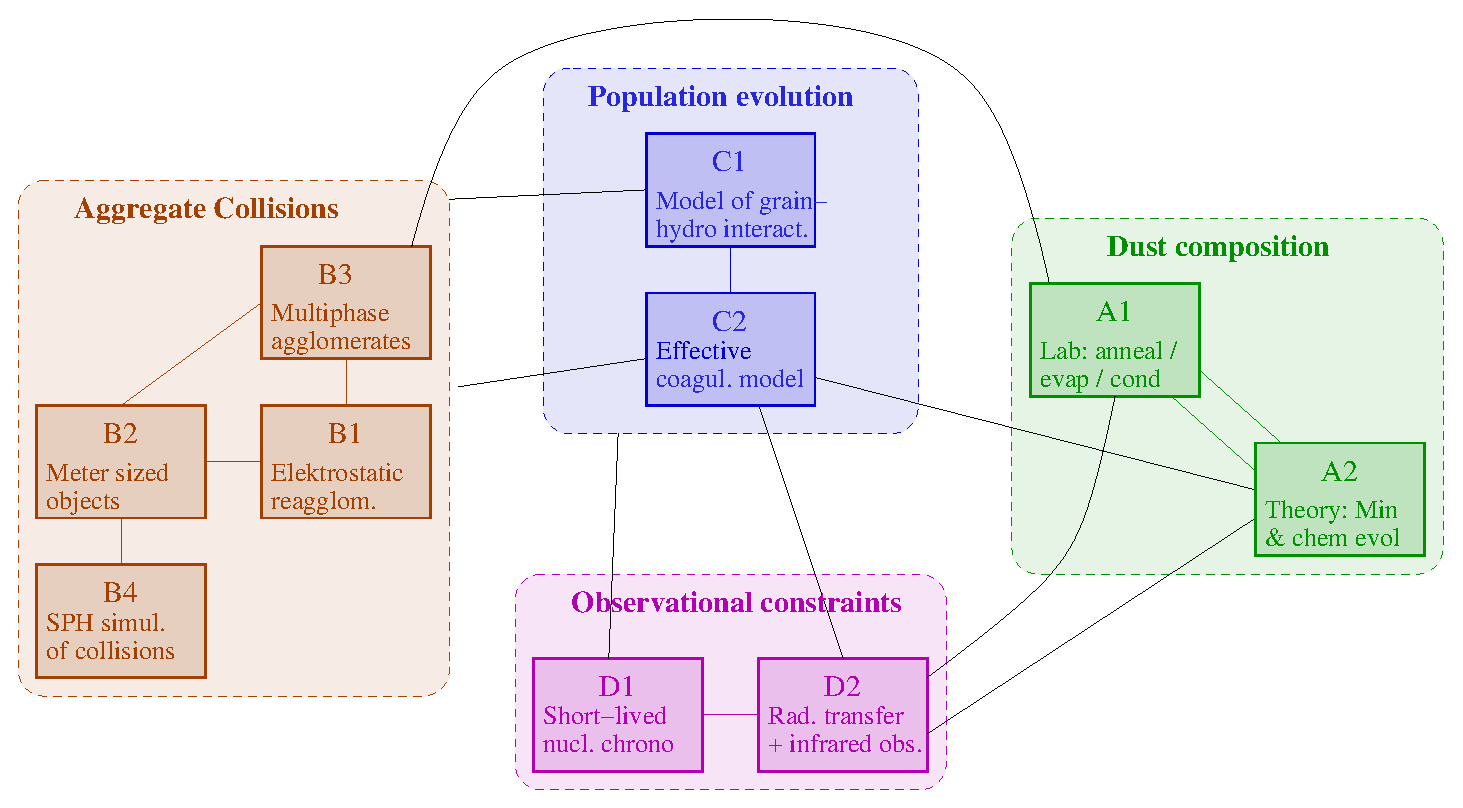
\includegraphics[width=16cm]{diagram.eps}}
%\vspace{1em}
%Fig 1: A diagram showing the links between the various
%projects. See text for details.\\
%
\centerline{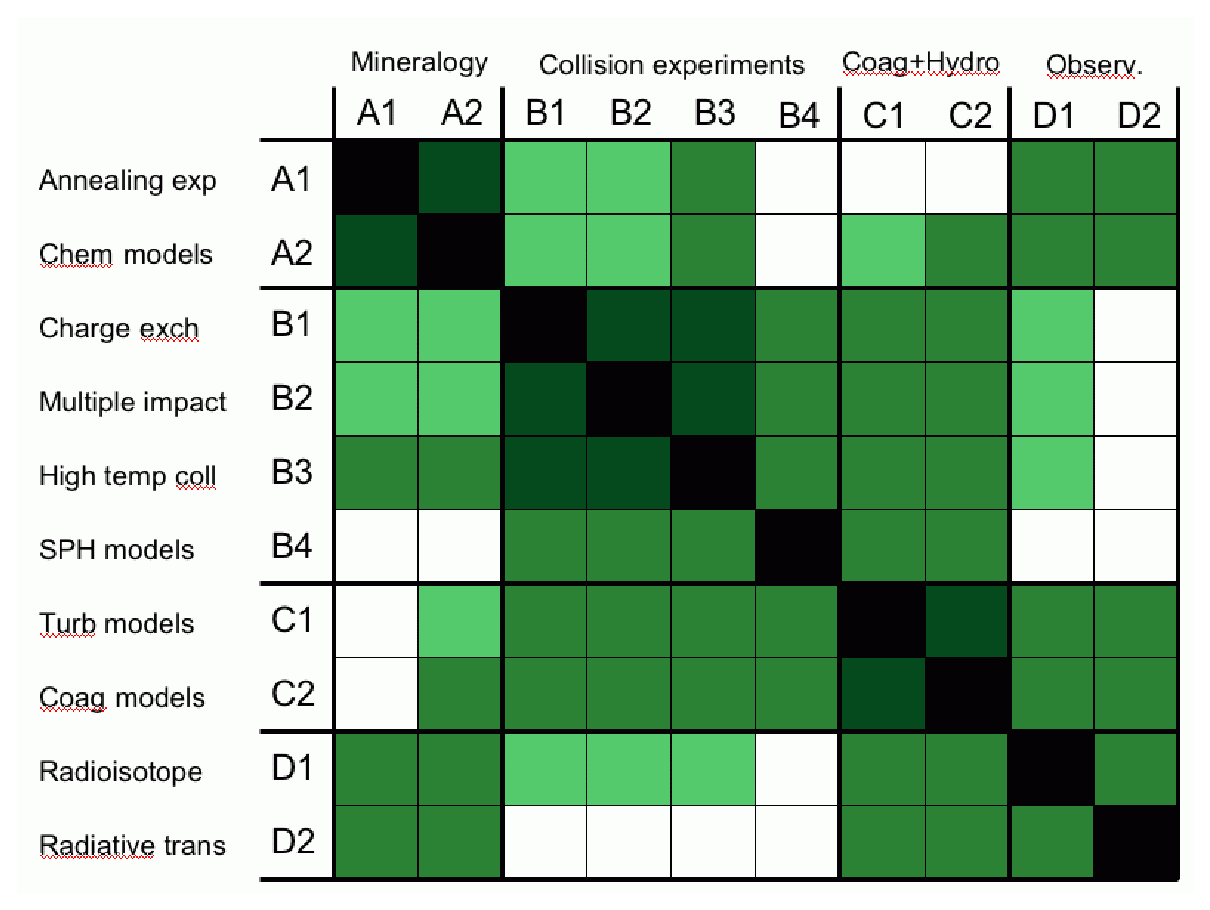
\includegraphics[width=12cm]{crosstable.eps}}
\vspace{1em}
Fig 1: A diagram showing the links between the various
projects. Dark-green means intense collaboration, on a
daily/weekly basis (5 links); intermediate green
means direct collaboration by exchange of data and iteration
between projects (23 links); light green means 
moderate collaboration, exchange of ideas (8 links). 
See text for details.\\
\vspace{2em}\mbox{}\\
\centerline{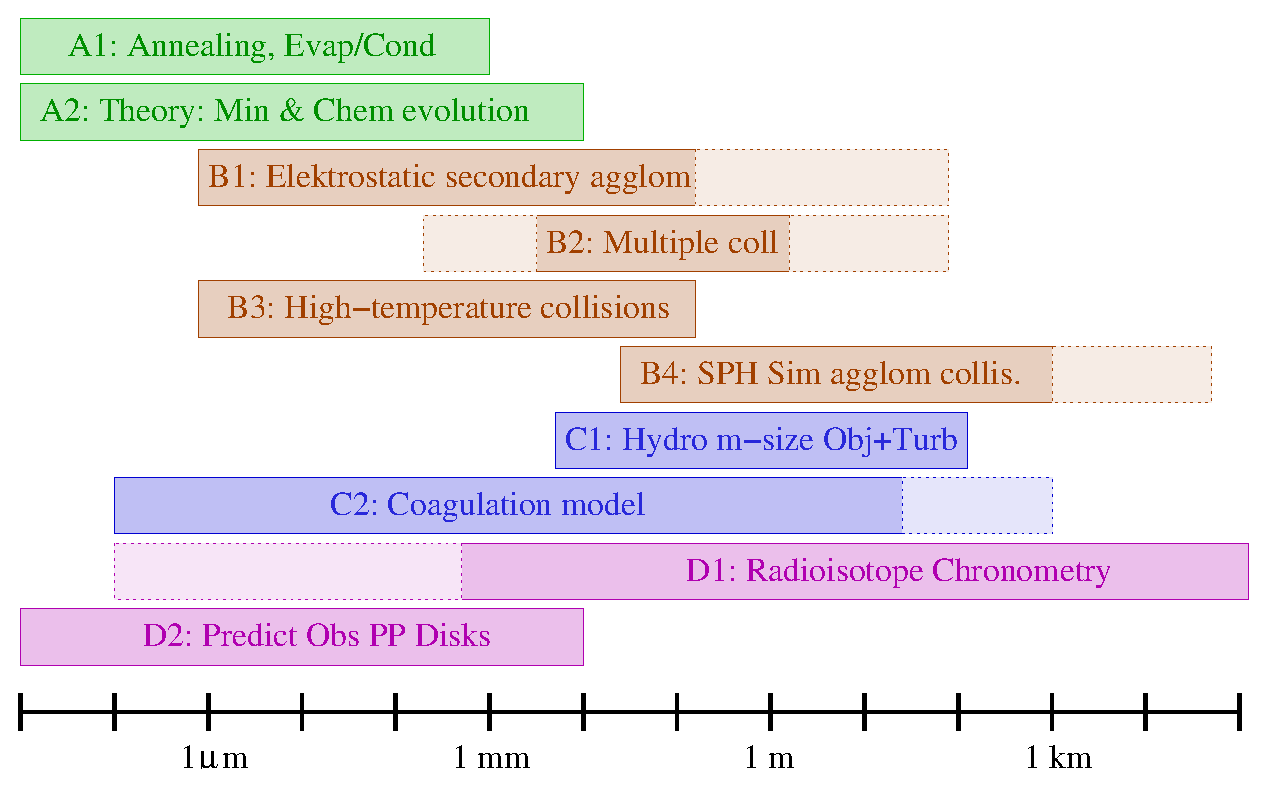
\includegraphics[width=16cm]{sizebar.eps}}
\vspace{1em}\\
Fig 2: A diagram showing the coverage
of the size-range between sub-micron dust particles and
multi-kilometer-sized planetesimals.
\end{figure}

\vspace{1.0em}

%
% Table with cross-connections
%
%\textbf{[***CHECK QUESTION MARKS BELOW***]}

% \newcommand{\chk}{$\surd$}
% \newcommand{\chkk}{$\surd\surd$}
% \begin{tabular}{l||cc|cccc|cc|cc}
%     &  A1  &  A2  &  B1  &  B2  &  B3  &  B4  &  C1  &  C2  &  D1  &  D2  \\
% \hline
% \hline
% A1  &      &\chkk &  .   &  .   & \chk &      &      &      & \chk & \chk \\
% A2  &\chkk &      &      &      & \chk &      &  ??  & \chk & \chk & \chk \\
% \hline
% B1  & \chk & \chk &      &\chkk &      & \chk & \chk &\chkk ?&     &      \\
% B2  &      &      &\chkk &      &      & \chk & \chk & \chk &      &      \\
% B3  & \chk & \chk &\chkk &\chkk &      & \chk & \chk & \chk &      &      \\
% B4  &      &      & \chk & \chk & \chk &      & \chk & \chk &      & \chk ?\\
% \hline
% C1  &      & \chk & \chk & \chk & \chk & \chk &      & \chk & \chk & \chk ?\\
% C2  &      & \chk & \chk & \chk & \chk & \chk &      &      & \chk & \chk \\
% \hline
% D1  &      & \chk & .?   & .?   & .?   & .?   & \chk & \chk &      & \chk \\
% D2  & \chk & \chk &      & \chk &      &      & \chk & \chk & \chk &      \\
% \hline
% \end{tabular}

\pagebreak[4]

\subsection*{\em Description of Scientific Blocks}
\vspace{0.5em}
In the following we present an overview of the contents of the four major
blocks in our Forschergruppe.
\vspace{0.8em}
 
\noindent\underline{{\bf Block \blockmineral{}:} Dust composition \& chemistry}
\vspace{0.8em}\\
%
%
The study of the composition and chemistry of solid material in
protoplanetary disks is required for the interpretation of infrared
observations of protoplanetary disks. 
% Without knowledge of dust composition
% and chemistry -- obtained from theoretical modeling and laboratory
% experiments -- it is difficult to extract information about the physical and
% chemical processes affecting the dust grains from the observed solid state
% features in the spectra of these protoplanetary disks.  
Such knowledge is also required for understanding the composition of comets,
asteroids, planets, including their atmospheres, oceans, and complex organic
materials.

In projects \projlattard{} and \projtscharn{} it is planned to investigate
the basic mineralogical and chemical processes that determine the properties
and the constituents of the dust mixture in protoplanetary disks. It will be
done for the first time in a consistent way by a joint interdisciplinary
effort of mineralogical laboratory investigations and astrophysical model
calculations.

The laboratory investigations in project \projlattard{} will analyze the
processes determining the composition and properties of the important
mineral components in the dust mixture. Presently, the most urgently needed
data for model calculations are realistic annealing data for interstellar
dust materials and vaporization/conden\-sa\-tion data for the dust materials
formed in the warm inner regions of accretion disks. Laboratory studies of
different groups have supplied already some data on silicate materials
(reviewed in Gail \cit{2003}) but important data are missing for
materials with the compositions expected to exist in protoplanetary disks.
In project \projlattard{} experiments will be performed on the
annealing and evaporation behavior of silicate compounds with varying
degrees of iron contents, which are expected to be the main dust
components. These experiments will provide the data required for realistic
models of the dust evolution in project \projtscharn{}. 
Vaporization and condensation experiments will be performed for the highly refractory
Calcium-Aluminum silicates for which hardly data are available yet.  These
experiments will be combined with an optical characterization of annealing
products and optical supervision of vaporization of thin films, which will
also supply optical data on important dust materials in temperature regions
not accessible to previous techniques, and they will provide necessary input data
for dust opacities, required in project \projwolf{}.

From the theoretical side we will (in project \projtscharn{}) approach this
problem by using a combination of modeling components. The structure and
evolution of the disk will be followed using time-dependent hydrodynamical models
coupled to a radiative transfer module. The chemistry of the solid and
gaseous components, as well as the physical and mineralogical processes
affecting the materials, will be modeled by extending previous work (Gail
\cit{2001, 2004}; Wehrstedt \& Gail \cit{2003}). Numerical tools for
calculating the structure and evolution of the disk with radiative transfer
(so far in the Eddington approximation, but extendible) are already
available, as well as subroutines for modeling transport processes and
chemical and mineralogical processes. Within the proposed project emphasis
is placed on the development of detailed chemical models for the chemical
evolution of the dust grains in the inner disk as well as on the formation
of ice coatings of grains in the outer disk regions. For both of these
aspects it is necessary to also model gas-phase chemistry in order to
predict the composition of the condensates.

The outcome of the models will provide important input-information required in
science block \blockimpact{} and project \projdul{} by specifying the
expected chemical composition of the colliding dust aggregates. Also it
predicts the abundances of certain minerals in protoplanetary disks, which are
required as input for radiative transfer modeling in project \projwolf{}.
The project needs input about general disk properties and evolutionary
timescales from projects \projtrie{} and \projwolf{}.
%

%\vspace{1em}\\

%\pagebreak[4]

%\noindent\underline{{\bf Block \blockimpact{}:} Collisions between dust
%aggregates}\\
%\mbox{}\vspace{1em}\\
\noindent\underline{{\bf Block \blockimpact{}:} Aggregate collisions}\\
%
The growth of dust from micrometer-sized particles to km-sized planetesimals
is a process involving a large sequence of individual collisions between
pairs of dust agglomerates. Whether such collisions lead to coalescence or
fragmentation depends on many parameters including the impact velocity and
the structure and composition of the aggregates involved. Laboratory
experiments have, over the past couple of years, yielded considerable
insight in the outcomes of such collisions, but large uncertainties
remain. These uncertainties include in particular collisions between bodies
exceeding a few cm in size and collisions between bodies of very different
sizes. In order to understand whether (and how) bodies can grow beyond the
`meter size barrier' the regime of high impact velocities and/or large
bodies must be studied in the laboratory and by using numerical
simulations. Two projects of block B intend to study the collisions of
aggregates in these new size regimes. The other two projects aim to study
additional effects of charge, temperature and composition on particle
growth. The laboratory experiments will be based on the huge progress in
experimental techniques of handling large monolithic dust samples and of
generating collisions between individual dust particles.
% 
% This will extensively broaden our knowledge of the outcomes of such
% collisions, with relevance to the formation stage of planetesimals.
%

In project \projblum{} we will study the role of charge separation during
collisions between small and large bodies on the growth process. A
succession of non-sticking collisions can lead to the build-up of strong
electric fields on the larger bodies from which emerging, previously
non-sticking dust particles are not able to escape. This project aims at the
experimental test of this concept and the modeling of the charge-induced
growth of planetesimals.

In project \projwurm{} laboratory experiments will be carried out with large
($>$ dm-sized) dust agglomerates subject to multiple collisions. It will be
studied if and how such agglomerates compactify, whether collisions lead to
growth or fragmentation, and whether debris products can re-accrete onto the
main body by hydrodynamic friction. The role of elastic waves and porosity
will be studied.

% The role of compaction, dilution, fragmentation, elastic waves, ejection 
% and re-accretion of material will be studied. 

In project B3 the collision experiments shall be extended to mineral phases
(Mg, Ca, Al silicates) that are expected from theoretical and observational
-- both astrophysical and cosmochemical -- constraints in protoplanetary
disks.  Particularly effects at high temperatures and dust/gas ratios
(sintering, eutectic melting between immiscible phases) could be key
mechanisms to trigger agglomerate growth beyond previously established
critical sizes (dm/m) and collision velocities (few m/s).

Parallel to the laboratory collision experiments, we will
(in project \projkley{}) perform numerical
simulations to determine the outcome of individual collisions between
aggregates. For this purpose an existing {\em Smooth Particle Hydrodynamics}
code for modelling elasto-plastic media will be adapted and 
calibrated with the laboratory data. With this code,
extrapolations on the collisional growth of dust aggregates to much larger
sizes will be possible and will allow the development of a realistic model
of planetesimal formation.

The embedding of these projects within the proposed Forschergruppe, in
particular the connection with science blocks \blockmineral{} and
\blockglobal{}, is of fundamental importance. First of all, the use of
realistic silicate dust mixtures in project B3 (and in the course of the
projects also B1 and B2) is a direct combination of collision experiments
and mineralogy. It is investigated how complex mineralogical compositions of
aggregates influence the outcome of collisions. Second, all projects of
block \blockimpact{} connect directly to block \blockglobal{}. The main
input parameters for the collision experiments, such as aggregate type, size
(project \projdul{}), and impact velocity (project \projklahr{}), can only
be determined in close collaboration with the models of block \blockglobal{}.
% It only makes sense to model
% collisions between certain aggregates with certain impact velocities if such
% aggregates indeed exist under these conditions, and if they indeed collide
% with these velocities. 
Moreover, the results of block \blockimpact{} have their highest relevance
when they can be applied to  models that can simulate the dust evolution on
a global scale (block \blockglobal{}), to study the effect of the lab
findings on the global particle population.
%
% using statistical methods (project \projdul{}), and models
% that can follow the transport of roughly meter-sized bodies through the disk
% (project \projklahr{}). This post-experiment modeling can tell what the
% effects of the laboratory findings are on the evolution of the particle
% distribution.
%
% For instance: knowing from block \blockimpact{} that certain
% collisions are destructive raises the question whether, as a consequence of
% this, most bodies of that size regime indeed suffer at least one such
% destructive collision, and whether the dust population is thereby
% significantly affected -- a question that can only be answered with the
% projects of block \blockglobal{}.  Vice versa, important input from Block
% \blockglobal{} about collision velocities is required for the projects in
% Block \blockimpact{}.
%

%\pagebreak[4]

%
\mbox{}\vspace{1em}\\
\noindent\underline{{\bf Block \blockglobal{}:} Particle population evolution}\\
%
%
%
\noindent The growth from dust to planetesimals is a process involving
extremely large numbers of particles. Each particle has its own location in
the protoplanetary disk and moves with its own velocity. While science block
\blockimpact{} is concerned with collisions between individual particles,
science block \blockglobal{} is concerned with the behavior of the dust {\em
population}. There are two main aspects: the systematic and random movements
of the particles through the disk and the evolution of the size-distribution
of the particles. In the Forschergruppe there will be a project to address
the first issue (project \projklahr{}) and a project to address the second
issue (project \projdul{}). 

In project \projklahr{} the movement of swarms of dust particles is modeled
with full magneto-hydrodynamics models.  This allows us to determine the
random and systematic motion of particles of different sizes, and thus
determine how often particles collide, and with which velocities. This is a
{\em fundamental} input parameter to dust coagulation models, and will be of
crucial importance to all the projects of block \blockimpact{}, as well as
to project \projdul{}. Additionally, it will be studied in this project
whether turbulence and vortices can concentrate the dust particles in small
regions which enhance the probability that they collide. With project
\projwolf{} it will be investigated if such concentrations can be observed in 
millimeter observations in the outer regions of protoplanetary disks.

In project \projdul{} we will develop a global coagulation model which solves
the evolution of the dust grain size distribution as a function of time and
location in the disk. This project is aimed at unifying the results of the
Forschergruppe into a single model, albeit with many simplifications to keep
the problem tractable. Outcomes from the various projects of the
Forschergruppe will be parameterized, tabulated or approximated by fitting
formulae, so that they can be incorporated into the model of project
\projdul{}, and the interconnection between all these processes be
investigated. This `effective model' will allow us to see what the effect of
all the microphysics from block \blockimpact{} and the mineralogy from block
\blockmineral{} is on the evolution of the particle population in
general. This can subsequently be channeled into the radiative transfer
modeling of project \projwolf{} to make observational predictions and allow
direct comparison to the observations.

%\pagebreak[4]


\mbox{}\vspace{1em}\\
\noindent\underline{{\bf Block \blockobserv{}:} Observational constraints}\\
%
\noindent Science block D has the aim of developing the interface between
the Forschergruppe and two main scientific fields that empirically constrain
the formation and growth of planetesimals. This will be in the form of
comparison to infrared/sub-millimeter observations of protoplanetary disks
and in the form of comparison to meteoritic data.

Infrared observations of protoplanetary disks yield data about if/where in
the disk certain dust mineralogical species at certain grain sizes reside.
The coagulation models (project \projdul{}), with input physics from
the collision experiments (block \blockimpact{}), yield predictions on the
expected life time of small dust grains in the disk and their average sizes.
The mineralogical/chemical models of project \projtscharn{} will predict the
thermal processing history of the dust and the radial mixing of these
various dust species. These models will yield the 2D and 3D grain
size/property distribution as a function of time, which can
directly be inserted in a radiative transfer code (project \projwolf{}) to
produce predictions for the spectral energy distributions {\em and} the
solid-state spectral features of these spectra.

While infrared observations give important information about growth
processes from micrometer to millimeter scales, another important
observational constraint on planetesimal formation is the timing of growth
from millimeter to 100 km size objects. For our own Solar System dating of
meteorite constituents can provide details with the time resolution of
better than a few hundred thousand years, by using long and short-lived
nuclide chronometry (Lugmair \& Shukolyukov \cit{1998}; Brazzle et
al.~\cit{1999}; Bizzarro et al.~\cit{2004}; Russell et~al.~\cit{1996}; Kita
et~al.~\cit{2000}; Trieloff et al.~\cit{2003}; Trieloff \& Palme
\cit{2006}).

In the case of the infrared observations (project \projwolf{}) the MPIA
already has the data-reduction and first-order interpretation of these data
as one of its main scientific activities. The (project \projwolf{}) aims to
connect the main activity of the Forschergruppe and the results from the
infrared observers at MPIA and in general. Additional help with this
interpretation will be given by other members of the Forschergruppe with
experience in comparing complex models to observations. In the case of
comparison to meteoritic data it must be kept in mind that this field is
already quite mature, and an enormous volume of knowledge is already
present. Comparison to this data can be done by the students from other
projects in close collaboration with the mineralogists of the
Forschergruppe. The proposed project on nuclide chronometry deals with the
key question of the timing of chondrule and planetesimal formation (Trieloff
\& Palme \cit{2006}), i.e. if chondrule formation is closely associated in
time and space to parent body formation with each parent body forming fast
(within a few 100\,000 years) from a restricted zone, or if chondrule
forming processes and subsequent incorporation into planetesimals allows
time for radial mixing of chondrules between different zones of the early
solar nebula.  
%
In another part of project D1, laboratory analysis of cometary dust samples
returned by the STARDUST mission will aim at quantifying the fraction of
material that experienced high temperature annealing, metamorphism,
condensation or evaporation and was transported outwards by radial mixing
processes into comet forming regions.


%% \mbox{}\vspace{1em}\\

\subsection*{\em Milestones}
\vspace{0.5em}
%
%%\mbox{}\vspace{1em}\\
%%\noindent{\bf \em Milestones}\vspace{0.8em}\\
%
\noindent The first 1.5 years will be a start-up phase: laboratory experiments will
be set up, numerical codes designed and first results booked (see below). During
this period, the collaboration between (and within) the individual projects is aimed
primarily at a transfer of know-how and expertise. After about 1.5 years, when
first results are expected, the focus of collaboration will gradually shift
to the exchange of results (i.e.~the results of one project being the input
to another). The main scientific objectives will then be targeted.

{\em Milestones block A:} In the startup phase we wish to obtain lab results
on Fe-bearing silicates, and first data on Ca,Al compounds. A first version
of disk models with gas phase and solid state chemistry will be developed.
In the second phase lab results from \projlattard{} will be used in
\projtscharn{}, model predictions on the location of crystalline silicates in
disks will be exported to \projwolf{}. Subroutines for solid state chemistry
and coagulation will be exchanged with \projdul{}. We expect to be able to
answer whether radial mixing theories can explain the variable composition
of volatile and refractory elements in our own Solar System and the
observational data on crystalline silicates in protoplanetary disks. 

% The
% issue to explain oxygen isotopic compositions of chondrites is certainly
% more challenging, and may be addressed in a possible extension of the
% Forschergruppe.

{\em Milestones block B:} In the initial phase existing experimental setups
will be modified, e.g.~implementing charge-transfer measurement equipment
for \projblum{} and preparation of multi-phase agglomerates for
\projblumtrie{}. The main measuring phase can already start after about 9
months. First data (e.g.~growth/erosion rates of charged impacts
(\projblum{}) / porous objects (\projwurm{}), sticking coefficients of
multi-phase agglomerates (\projblumtrie{})) will be transferred to other
blocks after about 1.5 years, and refined in the following years. The
numerical modeling of project \projkley{} will start with the implementation
of a more detailed porosity model in the existing SPH code,
and comparison and validation against
the lab experiments of block \blockimpact{}. In the second half of the
project a survey will be conducted of two-body aggregate collisions of
sizes larger than reachable in the laboratory. These data will then be
transmitted to other projects after about 2 years. 


{\em Milestones block C:} Due to the challenging nature of the hydrodynamic
simulations of project \projklahr{}, the first 1.5 years will be spent
mainly on the development and testing of the numerical tools such as radiative
transport in the diffusion approximation. First
realistic estimates of collision velocities and rates, as well as transport
of particles are expected by this time, and transmitted to science block
\blockimpact{} over the next 1.5 years. For project \projdul{} we will first
develop recipes for implementing experimental results into the coagulation
code. This will involve an extra `dimension' (dust property). At first we
will use already available lab data, and by about 1.5 years the new data
from the Forschergruppe will be implemented. The focus will then shift to
the application of the models to solving the outstanding scientific
questions mentioned in the project description.


{\em Milestones block D:} Project \projtrie{}: In the startup phase we aim
to obtain first chronological results (I-Xe, Al-Mg) on a first series of
chondrules from ordinary and carbonaceous chondrites. The most promising
meteorites will be selected in the second phase, in order to check the
relative timing of chondrule and chondrite formation. We expect constraints
on possible radial mixing processes of chondrules in the disk, and hints at
possible processes that speed up or delay planetesimal formation. 
%
From Stardust analysis the preliminary examination phase should allow a
rough estimate of the fraction of high temperature material found in comets.
%
Project \projwolf{}: In the first half existing models of
circumstellar disks will be used to study the influence of various disk and
dust parameters on observable quantities. As the project proceeds, new
results from the Forschergruppe will be considered and the disk models
improved accordingly. By this time the dust production by collisions of
planetesimals will be added to the models.



% Examples of such output-input exchange are:
% using collision velocity predictions from hydrodynamic simulations in lab
% experiments, taking into account the results from lab collision experiments
% and theory in coagulation models, using new lab data of thermal processing
% of minerals in theoretical models, using refined models of dust evolution
% and transport in disks for radiative transfer models for infrared spectra.

\subsection*{\em Future perspectives}
%%\mbox{}\vspace{1em}\\
%%\noindent{\bf \em Future perspectives}\vspace{0.8em}\\
%
This Forschergruppe proposal is focused entirely on the initial growth phase
of planets. 
Even though we hope to make good progress within the coming 3 years 
there will be probably more than enough open points and refinements for a
continuation of this work in the following funding period.
Additionally, we may envision to extend the focus and 
include studies of gravitational clustering of planetesimals, the capturing
of gas by protoplanets and the eventual formation of rocky and gas giant
planets. 
By that time major new developments are expected in the field of
observations of extrasolar planets which can constrain our models.


\section{Preconditions of the Forschergruppe}
\subsection*{\em In-house activities on meteoritics and observational astronomy}
%
%%\mbox{}\vspace{1em}\\
%%\noindent{\bf \em In-house activities on meteoritics and observational
%%astronomy}\vspace{0.8em}\\
%
Science block D has the aim of developing the interface between the
Forschergruppe and two main scientific fields that empirically constrain the
formation and growth of planetesimals. These fields are already strongly
represented by our current research:
%
\begin{itemize}
%
\item {\bf Composition of meteorites}\\
%
The wealth of data available from meteoritic and planetary science,
including aspects of mineralogy, isotope chronology, cosmochemistry and
geology needs to be incorporated into astrophysical models. Specific studies
related to the early evolution of meteorite parent bodies (M.~Trieloff), as
well as general experience in analytical and experimental mineralogy and
petrology (D.~Lattard, R.~Altherr) will guarantee the transfer of
geoscientific aspects into the interdisciplinary projects of the
Forschergruppe.

\item {\bf Observations of protoplanetary disks:}\\
%
In spite of the enormous surge in observational data of protoplanetary disks
currently arriving from e.g.~the Spitzer Space Telescope, the Very Large
Telescope and other facilities, our Forschergruppe does not require
personnel for the acquisition, reduction and first analysis of these
data. The MPIA has a large team of scientists dedicated to this task, and
the involvement of the MPIA in the Forschergruppe guarantees access to large
quantities of reduced and directly useable data. 
%Some members of the
%Forschergruppe (S.~Wolf, Th.~Henning and C.P.~Dullemond) have strong
%connections to the observational community both inside the MPIA and outside.
\end{itemize}

%
% 
\subsection*{\em Past and current activities}
The planned activities of the proposed Forschergruppe are part of an
increased scientific interest in the area of planet formation in Germany.

For several years now the contacts between the geophysical/mineralogical and
astrophysical scientific communities in Germany have intensified, mainly
through the organization of a series of ``Planet Formation'' workshops,
specifically meant to create a platform for discussion and interaction
across fields.  These were held over the past 5 years in Berlin, Weimar,
M\"unster and most recently in Heidelberg (this March).  The last two
meetings of this series have been organized by members of the proposed
Forschergruppe: G.~Wurm (PI of project B2), S.~Wolf (PI of project D2) and
M.~Trieloff (Co-Speaker of this Forschergruppe), and the next workshop is
planned to take place in 2007 in Braunschweig (organized by J.~Blum, PI of
projects B1 and B3).

At the same time the Max-Planck-Institute for Astronomy in Heidelberg has
organized several international workshops on very closely related
fields. The latest one was on Planet Formation in Ringberg, December 2004,
organized by H.~Klahr (PI of project C1) and W.~Brandner, from which a book
will soon published by Cambridge University Press. The next meeting,
organized by C.P.~Dullemond (Co-Speaker of this Forschergruppe) together
with H.~Klahr (PI project C1), has a topic very close to that of the
Forschergruppe: ``From Dust to Planetesimals'' and will be held in the very
near future (September 11-15, 2006) at Schlo{\ss} Ringberg.

In October 2005, S.~Wolf (PI of project D2) has organized a Heraeus School in
the field of Planet Formation, where many of the members of the FG have
given review talks about the status of the field and their own work related
to planet formation.

This short overview over activities in the field of Planet Formation in
Germany demonstrates clearly that {\it i)} interaction between the involved
scientists has taken place already, and that {\it ii)} there is rising
interest to combine efforts, and team-up to resolve scientific problems in close
collaboration.

\section{Education, communication and logistics of the Forschergruppe}
%
The sub-projects proposed in this Forschergruppen-proposal will be carried out
exclusively by PhD students under the supervision of the PIs of the
sub-projects. The topic of planetesimal formation is a modern, flourishing
and multi-disciplinary field of science in which the PIs of our proposed
Forschergruppe can -- and will -- provide an excellent and stimulating
working environment for the PhD students.

We propose 10 projects, with (in total) 13 PhD positions. Of those 13
positions, 11 are planned to be financed by the DFG (through the
Forschergruppe) while 2 PhD positions will be financed by the participating
institutes.

One of the pillars of our proposed Forschergruppe is the collaboration and
communication between the various teams. Some PhD students will have
advisors at different institutions and even at different locations. In other
cases the main work is done in one institute, but strong interaction is
required with the other institutions. For this reason we intend to include a
relatively large travel budget in our proposal. Each PhD student should have
the possibility to spend three weeks per year on a work visit in one of the
other nodes or up to three weeks in total spread over multiple work visits
to various nodes. For some of the PhD students, in particular those which
are shared by two institutes, longer work visits should be possible.

Regular small informal meetings will be organized between a subset of the
groups. Travel possibilities should be available for regular spontaneous
one- or two-day meetings of about 4 to 6 persons: e.g.~two collaborating PhD
students and their respective advisors.

%In addition to this we intend to invite international guests for one- or
%two-week visits to one--but preferably more--of the institutes of the
%Forschergruppe.

We intend to set up a bi-weekly Forschergruppe-Seminar, using
video-confe\-rencing methods. In each of these seminars, one of the PhD
students will report his/her latest developments, and in the rest of the
time there will be room for general discussion.

Twice a year a full group meeting of 3 days will be organized, starting
from the beginning of the second year.   These
meetings will be organized in a quiet isolated environment and will be half
in the form of talks and half entirely informal, providing sufficient time
for discussions.  During these meetings it will be possible to improve
connections and to focus on the target issues of the Forschergruppe. We
intend to invite one or two internationally acclaimed guests to these
meetings to give guest lectures on topics of common interest within the
Forschergruppe. The visit of these guests can/will be extended with a 1 week
visit to one or more of the nodes.

After the first half year, roughly summer 2007, a summer school will be
organized which covers all the topics of the Forschergruppe. This is
essential in order to guarantee that each student has a good enough level of
knowledge of the relatively broad interdisciplinary field covered by the
Forschergruppe, such that the planned interactions between the projects will be
successful. Although the primary focus will clearly be on the PhD students
of the Forschergruppe, the school will be open to all astronomy PhD students
from Germany and abroad. We will also invite international lecturers 
with an outstanding reputation.

\section{Forschergruppen-Professur}
%
One of the major goals of the proposed Forschergruppe is the initiation of
a close collaboration of researchers from different scientific communities
to jointly study the formation of planets around solar type stars.
At the heart of this effort lies the combination of geological/mineralogical
research with astronomy and astrophysics.  
This aim of our research group can be realized best through the creation of
a new Forschergruppen-Professur in the area of 
``Geoscientific and Astrophysical Planetary Research''. 
Heidelberg, where the main part of this Forschergruppe is localized,
constitutes the ideal location to create such a professorship.
The University of Heidelberg has prepared plans on how to announce and fill such
a professorship.
A more detailed justification of the requested position is given in project P. 
%

\newpage
\renewcommand{\hdrtitle}{Financial Overview}
\section{Financial Overview}
The total funds requested in all categories for all 10 projects are
summarized in the following tables (all amounts in \EUR).
%

\medskip

\subsection*{Personnel}
In all scientific projects the requested positions refer to
PhD students, where we ask for funding for 11 positions. 
The salary level refers to E13/2 (formerly Bat IIa/2). 
Two further PhD
positions (in projects A2 and C1) are funded by the ITA and the MPIA. 
These are denoted by (1/2) in table below.

\noindent
In project A1 and D1 additional funds are requested for
student research assistants (HiWis) for two
years to support the experimental work.
\\[0.2cm]
%
\centerline{\begin{tabular}{||l|r|r|r||}
\hline \hline 
 Project  & Year 1 & Year 2 & Year 3 \\ \hline %
 A1       & 56.500  & 56.500  & 48.000  \\
 A2 (1/2) & 24.000  & 24.000  & 24.000  \\
 B1       & 24.000  & 24.000  & 24.000  \\
 B2       & 24.000  & 24.000  & 24.000  \\
 B3       & 24.000  & 24.000  & 24.000  \\
 B4       & 24.000  & 24.000  & 24.000  \\
 C1 (1/2) & 24.000  & 24.000  & 24.000  \\
 C2       & 24.000  & 24.000  & 24.000  \\
 D1       & 28.500  & 26.250  & 24.000  \\
 D2       & 24.000  & 24.000  & 24.000  \\
\hline
{\bf Total:} (EUR)       & 277.000  & 274.750 & 264.000 \\
\hline \hline
\end{tabular}
}

\vspace{2.0cm}

%
\subsection*{Consumables}
The amounts for consumables refer primarily to materials that
have to used in the experimental studies.
\\[0.2cm]
% 
\centerline{\begin{tabular}{||l|r|r|r||}
\hline \hline
 Project  & Year 1 & Year 2 & Year 3 \\ \hline %
 A1       & 16.250  & 16.250  & 10.000  \\
 A2       &    400  &    400  &    400  \\
 B1       &  9.000  &  7.000  &  6.000  \\
 B2       &  1.240  &  1.240  &  1.240  \\
 B3       &  8.408  &  8.000  &  7.000  \\
 B4       &   -     &   -     &   -     \\
 C1       &   -     &   -     &   -     \\
 C2       &   -     &   -     &   -     \\
 D1       &  8.300  &  8.300  &  4.800  \\
 D2       &   -     &   -     &   -     \\
\hline
{\bf Total:} (EUR)       &  43.598    & 41.190   &  29.440 \\
\hline \hline
\end{tabular}
}

\newpage
%
\subsection*{Travel}
The amounts for travel refers to money allocated directly to the
individual projects, first to support longer term visits between the
different closely collaborating nodes of the Forschergruppe, and second
expenditures related to experimental studies that have to
be conducted outside of the Forschergruppe. This money is in addition to
that in project Z.
\\[0.2cm]
% 
\centerline{\begin{tabular}{||l|r|r|r||}
\hline \hline 
 Project  & Year 1 & Year 2 & Year 3 \\ \hline %
 A1       &  4.046  &  4.046  &  1.368  \\
 A2       &  3.000  &  3.000  &  3.000  \\
 B1       &  4.000  &  5.600  &  5.600  \\
 B2       &  3.810  &  3.810  &  3.810  \\
 B3       &  5.100  &  6.700  &  6.700  \\
 B4       &  2.760  &  2.500  &    570  \\
 C1       &  2.820  &  2.820  &  2.820  \\
 C2       &  4.640  &  2.720  &  2.540  \\
 D1       &  6.129  &  6.129  &  1.356  \\
 D2       &  1.300  &  1.300  &  1.300  \\
\hline
{\bf Total:} (EUR) &   37.605   &   38.625 &    29.064  \\
\hline \hline
\end{tabular}
}

\vspace{2.0cm}

%
\subsection*{Small Equipment}
Investments necessary for carrying out the experiments.
\\[0.2cm]
%
\centerline{\begin{tabular}{||l|r|r|r||}
\hline \hline 
 Project  & Year 1 & Year 2 & Year 3 \\ \hline %
 A1       & 27.000  &   -     &   -     \\
 A2       &   -     &   -     &   -     \\
 B1       & 12.269  &   -     &   -     \\
 B2       &   -     &   -     &   -     \\
 B3       & 16.771  &  2.500  &   -     \\
 B4       &   -     &   -     &   -     \\
 C1       &   -     &   -     &   -     \\
 C2       &   -     &   -     &   -     \\
 D1       &   -     &   -     &   -     \\
 D2       &   -     &   -     &   -     \\
\hline
{\bf Total:} (EUR)       & 56.040  & 2.500 & - \\
\hline \hline
\end{tabular}
}

\newpage

%
\subsection*{Others costs}
Materials for experimental work and 
computer equipment in more theoretical studies.
\\[0.2cm]
%%
\centerline{\begin{tabular}{||l|r|r|r||}
\hline \hline
 Project  & Year 1 & Year 2 & Year 3 \\ \hline %
 A1       &  9.250  &  9.250  &  7.250  \\
 A2       &   -     &   -     &   -     \\
 B1       &   -     &   -     &   -     \\
 B2       &  1.000  &         &         \\
 B3       &   -     &   -     &   -     \\
 B4       &  2.000  &   -     &   -     \\
 C1       &  4.000  &   -     &   -     \\
 C2       &  2.000  &   -     &   -     \\
 D1       &  3.200  &  3.200  &   -     \\
 D2       &  2.000  &   -     &   -     \\
\hline
{\bf Total:} (EUR)       &   23.450    &  12.450    &   7.250    \\
\hline \hline
\end{tabular}
}

\medskip

%
\subsection*{Central Budget}
The total funds requested for Project Z are summarized in the following table.
\\[0.2cm]
\centerline{\begin{tabular}{||l|r|r|r||}
\hline \hline & Year 1 & Year 2 & Year 3 \\ \hline %
Networking                  & 24.800  & 41,800  & 41,800  \\
External Travels            & 30.000  & 30.000  & 30.000  \\
External Guests             & 30.000  & 30.000  & 30.000  \\
Conference/Summerschool     & 20.000  &   -     & 20.000  \\
Consumables                 &  1.000  &  1.000  &  1.000  \\
Publications                &  5.000  &  5.000  &  5.000  \\
Management    (Bat Vb/2)    & 21.000  & 21.000  & 21.000  \\
\hline
{\bf Total:} (EUR)          & 131.800  & 128.800 & 148.800 \\
\hline \hline
\end{tabular}
}

\medskip

%
\subsection*{\large Total Budget}
Listing of total costs
\\[0.2cm]
%
\centerline{\begin{tabular}{||l|r|r|r||}
\hline \hline
 Item              & Year 1 & Year 2 & Year 3 \\ \hline %
 Positions (PhD/HiWi)  & 277.000  & 274.750 & 264.000 \\
 Travel (projects)     &  37.605  &  38.625 &  29.064  \\
 Small Equipment       &  56.040  &   2.500 &   -     \\
 Consumables           &  43.598  &  41.190 &  29.440 \\
 Other Costs           &  23.450  &  12.450 &   7.250  \\
 Project P             &  80.000  &  80.000 &  80.000 \\
 Project Z             & 131.800  & 128.800 & 148.800 \\
\hline \hline
{\bf Total:} (EUR)     & 649.493  & 578.315 & 558.554  \\
\hline \hline 
\end{tabular} 
}

\newpage
%
\renewcommand{\hdrtitle}{Signatures}
\section{Signatures}
%
The project leaders have agreed to be responsible for the scientific
work of their projects.\\[0.4cm]
%
\noindent
The Speaker and co-Speakers of the Forschergruppe:\\[0.4cm]
% 
\noindent
{\it The Formation of Planets: The Critical First Growth Phase}
\\[1.0cm]
%
% \noindent
% \begin{tabular}{p{5.5cm}p{5.5cm}p{5.5cm}}
% Prof.\ Wilhelm Kley    &  Dr.\ Cornelis~P. Dullemond   &  Dr.\ Mario~Trieloff \\
% Institut f\"ur Astronomie  &  Max-Planck-Institut      &  Mineralogisches Institut  \\
% \& Astrophysik         &  f\"ur Astronomie             &  Universit\"at Heidelberg \\
% Universit\"at T\"ubingen & 69117 Heidelberg            &  69120 Heidelberg \\
% 72076  T\"ubingen  & & \\
% \vspace{1em} & & \\
% %
% T\"ubingen, May 30, 2006 & Heidelberg, May 30, 2006 & Heidelberg, May 30, 2006\\
% \vspace{1em} & & \\
% %
% 
\epsfig{file=signature_kley.eps,width=50mm} & & \\
% \vspace{1em} & & \\
% Wilhelm Kley & Cornelis P. Dullemond & Mario Trieloff \\
% \end{tabular}
% 
\noindent
Prof.\ Wilhelm Kley\\
Institut f\"ur Astronomie \& Astrophysik\\
Universit\"at T\"ubingen\\
72076  T\"ubingen\vspace{1em}\\

\noindent Dr.\ Cornelis~P. Dullemond\\
Max-Planck-Institut f\"ur Astronomie\\
69117 Heidelberg\vspace{1em}\\

\noindent Dr.\ Mario~Trieloff\\
Mineralogisches Institut\\
Universit\"at Heidelberg\\
69120 Heidelberg\vspace{4em}\\

\noindent T\"ubingen, May 30, 2006\\[1em]

\noindent\begin{tabular}{p{5.5cm}p{5.5cm}p{5.5cm}}

\epsfig{file=signature_kley.eps,width=50mm} & 

\epsfig{file=signature_dul.eps,width=50mm} & 

\epsfig{file=signature_trie.eps,width=50mm}\\
\vspace{1em} & & \\
Wilhelm Kley & Cornelis P. Dullemond & Mario Trieloff \\
\end{tabular}
% 



% Prof. Wilhelm Kley  \\
% Institut f\"ur Astronomie \& Astrophysik \\
% Universit\"at T\"ubingen \\
% 72076  T\"ubingen
% \\[2.5cm]
% 
% 
% T\"ubingen, May 30, 2006 
% 
% \medskip
% 
% 
\epsfig{file=signature_kley.eps,width=50mm}\\Wilhelm Kley


%
\vfill 
$~$


\pagebreak[4]

